\documentclass{article}
\usepackage{graphicx}
\usepackage{caption}
\usepackage{subcaption}
\usepackage[paper=a4paper,margin=1in]{geometry}
\usepackage[fontsize=12pt]{fontsize}
\usepackage{amsmath, amsthm, amssymb}
\usepackage[hidelinks]{hyperref}
\usepackage[nameinlink, noabbrev]{cleveref}
\usepackage{tikz}
\usepackage{booktabs}
\usetikzlibrary{arrows.meta}

\newtheorem{theorem}{Theorem}[section]
\DeclareMathOperator{\sgn}{sgn}

\title{Math 475 -- Project 3 \\ Modeling Pandemics}
\author{Jackson Brienen}
\date{November 7 2025}

\begin{document}

\maketitle

\section{Introduction}

Pandemics suck, not just for those who experience them, but also for the mathematicians and scientists tasked with quickly understanding and remedying their impact. In this paper we will discuss the basic yet powerful SIR model used for modeling pandemics. We will cover how the model works, the needed parameters for the model, how these parameters can affect a model, and how we can estimate said parameters by analyzing pandemic data.

\section{SIR Model}

The SIR model has three main equations, $S(t)$ representing susceptible individuals, $I(t)$ representing infected individuals, and $R(t)$ representing recovered individuals. With this come the following assumptions.

\begin{itemize}
    \item The total population, $N$, is constant, i.e. $S(t) + I(t) + R(t) = N$ for any $t$.
    \item Once an individual has recovered, they cannot be reinfected.
    \item The rate of transmission, denoted $\alpha$, is constant.
    \item The rate at which infected individuals recover, denoted $\beta$, is constant.
    \item Deaths count as recovery. So the recovery rate, $\beta$, is the rate for both people being cured and people dying.
\end{itemize}

With this we form a system of differential equations to represent the change in these three functions.

\begin{gather}
    S' = -\alpha SI \label{eq:sprime} \\
    I' = \alpha SI - \beta I \label{eq:iprime} \\
    R' = \beta I \label{eq:rprime}
\end{gather}

\Cref{eq:sprime} shows that the change in susceptible individuals is the rate of transmission applied to the number of interactions between susceptible and infected people. \Cref{eq:rprime} shows that the change in recovered individuals is the recovery rate applied to the number of infected people. Finally, \cref{eq:iprime} is the combination, adding the amount lost from susceptible to infected and taking away the amount recovered.%
\begin{figure}
    \centering
    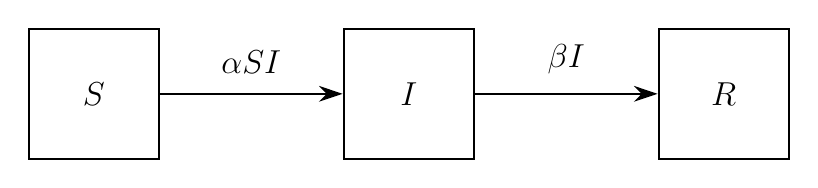
\begin{tikzpicture}
        % Define node styles
        \tikzstyle{compartment} = [draw, thick, rectangle, minimum width=4em, minimum height=4em, align=center]

        % Draw the nodes
        \node[compartment] (S) {$S$};
        \node[compartment, right of=S, xshift=3cm] (I) {$I$};
        \node[compartment, right of=I, xshift=3cm] (R) {$R$};

        \draw[-{Stealth[length=3mm, width=2mm]}, thick] (S) -- 
            node[above=1mm] {$\alpha SI$} (I);
            
        \draw[-{Stealth[length=3mm, width=2mm]}, thick] (I) -- 
            node[above=1mm] {$\beta I$} (R);
    \end{tikzpicture}
    \caption{Visualization of exchange between SIR compartments in SIR model.}
    \label{fig:exchange}
\end{figure}%
This idea where susceptible moves to infected, and infected moves to recovered is known as a compartmental model, and can be seen in \cref{fig:exchange}.

For the purposes of this paper, we will use this model as a percentage model, i.e. $N=1$, or $100\%$ of a population, later we will show how data given as population numbers can easily be translated into percentages. We will also see how using a percentage based model can make some arithmetic easier. Furthermore, we know our model stays true to our assumption that $N$ remains constant, as the sum of the derivatives is $0$, since we can write $I' = -S'-R'$ so adding $S'$ and $B'$ will obviously result in $0$.

\section{Initial Modeling}

In this section we will visually analyze the behavior of the model as parameters change. The two parameters we analyze are the rate of transmission, $\alpha$, and the recovery rate, $\beta$. 

\begin{figure}[h]
    \centering
    \includegraphics[width=.5\linewidth]{plots/simple.png}
    \caption{SIR Model with $N=1$, $I(0)=1/100$, $\alpha = 0.5$, and $\beta = 0.33$.}
    \label{fig:simple}
\end{figure}

As we can see in \cref{fig:simple}, in the long term, the system stabilizes. Eventually infected population drops to zero, and thus both $R'$ and $S'$ drop to zero. We can see in this case that roughly $60\%$ of the population was affected by the pandemic. We can actually solve for how these values are related. Simply we need to know, when our infected population reaches 0. But first, let's look at when the infectious decline begins, i.e. $I'=0$, which we see solved below.%
\begin{align*}
    0 &= \alpha SI - \beta I \\
    \alpha SI &= \beta I \\
    \alpha S &= \beta \\
    S &= \beta/\alpha
\end{align*}%
Thus, we can take our known $\beta$ and $\alpha$ and see that when $S=\frac{0.33}{0.5}=0.66$. Looking at \cref{fig:simple}, we see that when $S = 0.66$ we are at the peak of our infected population. Since we solved this generically, we can conclude that the peak of our infection will happen when our susceptible population reaches $\frac{\beta}{\alpha}$. This can help us conclude that relatively higher recovery rates, $\beta$ values, will lead to a less impactful pandemic, as well as higher transmission rates, $\alpha$ values, leading to more impactful pandemic.

Now, with a bit more work, we can find the exact point where we reach $I=0$. While directly solving the non-linear differential equations for this system is complex, we can instead solve the much simpler relation between \cref{eq:iprime,eq:sprime}.
\begin{align*}
    \frac{dI}{dS}&=\frac{\alpha SI - \beta I}{-\alpha SI} \\
                 &= \frac{\beta I}{\alpha SI} - 1 \\
                 &= \frac{\beta }{\alpha S} - 1 \\
              dI &= \left(\frac{\beta }{\alpha S} - 1 \right) dS \\
         \int dI &= \int \left(\frac{\beta }{\alpha S} - 1 \right) dS \\
              I  &= \frac{\beta}{\alpha}\ln(S)-S+C
\end{align*}
While we have this pesky integration constant, we can get solve for it by remembering the fact that before the pandemic $I=0$ and $S=1$ since $N=1$. In that case $0=\frac{\beta}{\alpha}\ln(1)-1+C$ which just means $C=1$. With this, we can now evaluate at $I=0$. While, this function can be solved, solving it is not practical or useful to us. Graphically though, this function is quite useful. Let's analyze this a few different $\beta/\alpha$ values.

\begin{figure}[h]
    \centering
    \includegraphics[width=.5\linewidth]{plots/solution.png}
    \caption{Solution of final $S$ value with differing $\alpha$ and $\beta$ values.}
    \label{fig:solution}
\end{figure}

As we see \cref{fig:solution}, if $0 < \frac{\beta}{\alpha} < 1$, our function intercepts at a value between $0$ and $1$. It also intercepts at $1$, but this is expected as that is how we solved for our integration constant. This intercept, is the final susceptible population after infected has hit zero. The blue line in the figure is using our $\alpha$ and $\beta$ values we previously plotted in \cref{fig:simple}. And we see the non-one intercept of the blue line, at around 0.375 in \cref{fig:solution} is roughly where our $S$ function levels out in \cref{fig:simple}. This intercept goes to $1$ as $\frac{\beta}{\alpha}$ approaches $1$ from $0$, and when ${\beta}{\alpha} = 1$, i.e. $\beta = \alpha$, there is only a single intercept at 1. This means, none of our population went to recovered, i.e. none of our population got infected. Obviously the reverse of this is true, as $\frac{\beta}{\alpha}$ approaches $0$, our ending susceptible population will also approach zero.

With this we can conclude, if $\beta$ stays constant, but $\alpha$ rises, the ending susceptible population will decrease. If $\alpha$ falls the ending susceptible population will increase. Similarly, if $\alpha$ is constant, but $\beta$ rises, the ending susceptible population will increase. If $\beta$ instead falls the ending susceptible population will decrease. And at any point $\alpha = \beta$, no one will get infected. Which makes sense since if someone gets infected and instantly recovers, the infection can't spread.

Let's take social distancing for example. During the COVID-19 pandemic, this act would directly affect the spread of the virus, i.e. $\alpha$ would decrease. While the recover time, does not change. With the conclusions made above, we know that this will cause the amount of ending susceptible individuals to increase. In other words, it reduced the total amount of people who got the virus. Let's use the previous example in \cref{fig:simple} but reduce $\alpha$ by half.

\begin{figure}[h]
    \centering
    \includegraphics[width=.5\linewidth]{plots/covid.png}
    \caption{SIR Model with $N=1$, $I(0)=1/100$, $\alpha = 0.25$, and $\beta = 0.33$.}
    \label{fig:covid}
\end{figure}

Comparing \cref{fig:simple,fig:covid}, we see that just reducing the transmission rate by half had a significant impact on how many individuals got the infection. Measures like masks, isolation, and other forms of protection against virus' will impact this $\alpha$ variable as well.

\newpage

\section{Data Analysis}

In this section we will use data to predict parameters in our model, to attempt to somewhat reflect the data. The data we will use in this section is as follows.

\begin{table}[ht]
\centering
\caption{Epidemic data for a small town ($N=250$).} % Optional: add a caption
\label{tab:epidemic_data} % Optional: for referencing
\begin{tabular}{@{}ccccc@{}}
\toprule
Time (in days) & Number of & Number of & Normalized & Normalized \\
elapsed & susceptible & infectives & susceptible & infectives \\ \midrule
0 & 235 & 15 & 0.94 & 0.06 \\
16 & 201 & 22 & 0.804 & 0.088 \\
31 & 154 & 29 & 0.616 & 0.116\\
47 & 121 & 21 & 0.484 & 0.084\\
62 & 108 & 8 & 0.432 & 0.032 \\
78 & 97 & 8 & 0.388 & 0.032 \\
109 & 83 & 0 & 0.332 & 0 \\ \bottomrule
\end{tabular}
\end{table}

Now to attempt to build an SIR model around this we must get two major variables, being $\alpha$ and $\beta$. We can use the same solution to our differential equation from the previous section $I=\frac{\beta}{\alpha}\ln(S)-S+1$ and, when $I=0$, but $S=0.332$ referencing \cref{tab:epidemic_data}, we can form a formula for either $\alpha$ or $\beta$, we will choose to form ours for $\alpha$.
\begin{equation}\label{eq:alpha}
    \alpha = \beta\frac{\ln(S)}{S-1}\approx1.651\beta
\end{equation}

With \cref{eq:alpha} we can take any $\beta$ and get an appropriate $\alpha$. But, since this only based on initial value, i.e. our starting point $I=0$ $S=N$, and an ending point $I=0$ $S=0.332$, our function may not line up exactly, but instead have a correct shape, i.e. starting and ending point. This is what we see happen if we use our previous $\beta = 0.33$

\begin{figure}[h]
    \centering
    \includegraphics[width=.5\linewidth]{plots/exp1.png}
    \caption{SIR Model with data from \cref{tab:epidemic_data}, $\alpha = $\ref{eq:alpha}, and $\beta = 0.33$.}
    \label{fig:exp1}
\end{figure}

As we see above, our estimated function is close for the initial and final data, and the general shape lines up, but the timeframe is way off. We can get an idea of how close we are through calculating the absolute error between our known data points, and the values predicted by our model. For the model in \cref{fig:exp1}, we find the sum absolute error for susceptible is roughly $1.2096$ and the sum absolute error for infected is roughly $0.2723$. These don't give us an idea of how close each is, but it does give us a metric which we can try to minimize.

\begin{figure}[h]
    \centering
    \includegraphics[width=.5\linewidth]{plots/exp2.png}
    \caption{SIR Model with data from \cref{tab:epidemic_data}, $\alpha = $\ref{eq:alpha}, and $\beta = 0.0734$.}
    \label{fig:exp2}
\end{figure}

Through iterative methods we can reduce our susceptible sum absolute error to $0.1110$ and our infected sum absolute error to $0.1676$, with $\beta = 0.0734$. This gives us the model in \cref{fig:exp2}. Which comparing \cref{fig:exp1,fig:exp2}, the latter is obviously a much closer fit.

\section{Conclusion}
In this paper, we explored the SIR model for pandemic modeling. We began by defining the model as a system of three differential equations. Through analysis, we demonstrated how the model's parameters, the transmission rate ($\alpha$) and the recovery rate ($\beta$), directly influence the pandemic's behavior. Specifically, the ratio $\beta/\alpha$ determines the peak of the infection and the total portion of the population that is affected. This connection provides a clear mathematical justification for public health measures like social distancing, which aim to reduce $\alpha$ and, as a result, lessen the pandemic's overall impact.

Furthermore, we demonstrated a practical application of the model by fitting it to a given dataset. By using the final state of the epidemic to establish an initial relationship between $\alpha$ and $\beta$, we were able to iteratively refine these parameters to find a model that closely matched the data. This process highlights how the SIR model, despite its simplicity, serves as a powerful and effective tool for understanding, analyzing, and predicting the outcome of an epidemic.


\end{document}